\chapter{Molecules Attract One Another Too}

\begin{kaichang}
While cooking, tear off some cling film, stretch it over a bowl, and smooth it around the rim. It sticks by itself, without glue or tape. Stranger still, you can peel it off, stick it back, and peel it again. What holds it on? And why is its grip so ``polite,'' releasing with one pull?

Before answering, consider these things. Why do morning dewdrops on grass form little balls instead of thin sheets? How can a gecko stroll upside down on a ceiling without suction cups or glue on its feet? Spray perfume indoors and minutes later the entire room smells of it, while the bottle's liquid dwindles day by day. Where did the escaped perfume go?

Four seemingly unrelated events. Guess whether they share one cause or have four separate causes. Record your guess and return at the end to check.
\end{kaichang}

\section{Sticking, Gathering into Balls, and Quietly Escaping}

First, line up the visible phenomena.

The first category is ``sticking'': cling film adheres to a bowl; two wet glass sheets are hard to separate; tape sticks to cardboard; chalk dust coats an eraser after wiping a board.

The second is ``gathering'': dew forms balls; a water strider stands without sinking, making only four dimples; a carefully placed paper clip floats on water; a falling tap stream narrows as though something pulls it inward.

The third is ``viscosity'': honey, syrup, and engine oil pour slowly, while water and alcohol rush out. Cold honey becomes even thicker, almost refusing to flow.

The fourth is ``escape'': hung-up wet clothes dry, alcohol on your hand feels cool and soon vanishes, and perfume silently ``flies'' throughout a room.

\begin{shiyan}
\textbf{How Many Drops Can a Coin Hold?}

Materials: a one-yuan coin, a dropper (or chopstick tip), clean water, and a drop of dishwashing liquid.

Procedure: lay the coin flat on a table and drip water onto its face. One drop, two, three---count while watching the surface bulge. Continue until it spills and record the count. Add a tiny drop of detergent to the remaining water, stir, dry the coin, and repeat.

What to observe: initially, water builds a small dome above the coin's edge without spilling. After adding detergent, the coin holds only a third as many drops or fewer, and the surface looks flattened.

Safety note: room-temperature water and one drop of detergent pose no danger; wipe the table afterward.
\end{shiyan}

What did the detergent do? It neither thinned the water nor shrank the coin. It disrupted a certain ``pull'' between water molecules, the protagonist of this chapter.

\section{Every Molecule Feels Its Neighbors' Pull}

Zoom in on a water surface. We know water and alcohol consist of molecules in ceaseless random motion, colliding and jostling. At the particle level, temperature measures average molecular speed: higher temperatures mean faster motion on average.

Imagine a molecule inside the liquid, surrounded by neighbors. Collisions from all directions roughly cancel, leaving it jostling locally. Now consider one at the \textbf{surface}: above is air, almost empty; below and beside it are companions. If it happens to acquire enough upward speed, it escapes as water vapor: evaporation. Vapor molecules flying in the air may also collide with the surface and be ``detained'' again: condensation. Clothes dry when departures outnumber returns.

\begin{center}
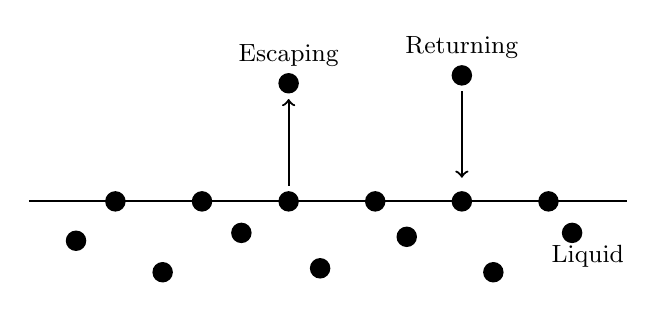
\begin{tikzpicture}[scale=1]
\draw[thick] (0,0) -- (7.6,0);
\foreach \x/\y in {0.6/-0.5, 1.7/-0.9, 2.7/-0.4, 3.7/-0.85, 4.8/-0.45, 5.9/-0.9, 6.9/-0.4}
  {\fill (\x,\y) circle (0.13);}
\foreach \x in {1.1, 2.2, 3.3, 4.4, 5.5, 6.6}
  {\fill (\x,0) circle (0.13);}
\draw[->,thick] (3.3,0.2) -- (3.3,1.3);
\fill (3.3,1.5) circle (0.13);
\draw[->,thick] (5.5,1.4) -- (5.5,0.3);
\fill (5.5,1.6) circle (0.13);
\node at (7.1,-0.7) {\small Liquid};
\node at (3.3,1.85) {\small Escaping};
\node at (5.5,1.95) {\small Returning};
\end{tikzpicture}
\end{center}

This is a representation: dots denote molecules, not their actual sizes or colors, and arrows show only motion directions.

Understanding evaporation explains alcohol's cooling effect on your hand. The fastest, most energetic molecules escape first, reducing the remaining molecules' average speed and temperature, so your skin supplies heat. Dogs panting and humans sweating likewise exploit ``evaporation carries energy away'' for cooling. Chapter 27 revisits the energy accounts.

Evaporation shows that liquid molecules pull one another. Without this restraint, every liquid would instantly disperse like spilled gas. But what is the pull? Not chemical bonding: Chapter 17 explained that bond formation and breaking alter molecules themselves, whereas evaporated water remains water and condenses when cooled, without a molecule being dismantled. Between molecules is a \textbf{real attraction much weaker than chemical bonds}. Weak enough to release when peeled, as with cling film, yet strong enough to gather hundreds of quadrillions of molecules into liquids and solids.

\section{Three Ways to ``Hold Hands''}

Intermolecular attraction involves not one but three ways of ``holding hands,'' differing in strength. All are fundamentally electromagnetic attractions between charges, with different charge-distribution patterns.

\subsection{Dispersion: Even ``Insular Households'' Cannot Escape}

Consider an apparent contradiction. Helium's outer shell is full and ignores others (Chapter 10), and methane, \chem{CH_4}, is nonpolar. Yet helium liquefies at $-269\,^{\circ}\mathrm{C}$ and methane at $-161\,^{\circ}\mathrm{C}$. \textbf{Every atom and every molecule attracts others, without exception.}

The origin lies in electrons. An electron cloud is not motionless candy floss; it fluctuates continually. For an instant, electrons may favor a molecule's left side, making it negative and the right positive: a fleeting ``temporary pole.'' This induces a neighboring cloud to shift, and the instantaneous dipoles attract. Their directions change the next instant, but attraction continues. Attraction from instantaneous cloud fluctuations is \textbf{dispersion force}, also called London force. Individually tiny, it is never absent.

One highly useful rule follows: \textbf{more electrons and larger molecules mean more easily distorted clouds and stronger dispersion}. The elemental halogen family supplies evidence:

\begin{table}[htbp]
\centering
\begin{tabular}{lccc}
\toprule
Substance & Electrons per molecule & Boiling point & State at $25\,^{\circ}\mathrm{C}$ \\
\midrule
Fluorine \chem{F_2} & 18 & $-188\,^{\circ}\mathrm{C}$ & Gas \\
Chlorine \chem{Cl_2} & 34 & $-34\,^{\circ}\mathrm{C}$ & Gas \\
Bromine \chem{Br_2} & 70 & $59\,^{\circ}\mathrm{C}$ & Liquid \\
Iodine \chem{I_2} & 106 & $184\,^{\circ}\mathrm{C}$ & Solid \\
\bottomrule
\end{tabular}
\end{table}

All four have the same structure---two identical atoms holding hands, with no permanent polarity. The only difference is increasing electron count. They progress from gas to solid as stronger dispersion eventually holds iodine molecules in a room-temperature solid. Noble gases follow the same sequence: helium, neon, argon, krypton, xenon, with boiling points climbing from $-269\,^{\circ}\mathrm{C}$ to $-108\,^{\circ}\mathrm{C}$.

An everyday example: natural gas's methane (one carbon) is gaseous; lighter fuel's butane (four carbons) liquefies under slight pressure; candle paraffin (twenty or thirty carbons) is solid at room temperature. All are hydrocarbon chains relying on dispersion, differing only in molecular size. Cling film also adheres through its long chains' dispersion forces, engineered to be weak and uniform enough for easy peeling.

\subsection{Dipole--Dipole: Molecules with Permanent ``North and South Poles''}

Chapter 20 explained that bent water has a negative oxygen end and positive hydrogen end, like a tiny magnet. Carbon dioxide has polar bonds but a symmetric line that cancels its poles, leaving it nonpolar overall. Molecules with permanent positive and negative ends, like water, line up: your positive end faces my negative, and mine faces the next molecule's negative. Attraction between permanent dipoles is \textbf{dipole--dipole interaction}, generally stronger than dispersion.

A direct comparison: acetone, the main ingredient in nail-polish remover, and butane have almost identical molecular sizes and electron counts, hence similar dispersion. But acetone has a permanent dipole and boils at $56\,^{\circ}\mathrm{C}$, while butane boils at only $-0.5\,^{\circ}\mathrm{C}$. Those extra degrees reflect the dipole--dipole ``bonus.''

\subsection{Hydrogen Bonds: Dipole Interactions' ``Special Forces''}

Something special happens when hydrogen bonds to highly electronegative nitrogen, oxygen, or fluorine (Chapter 11). Its sole electron is almost entirely pulled toward its neighbor, leaving its nucleus---a lone proton---half-exposed on the molecular surface with a strong positive charge. Electron-rich nitrogen, oxygen, or fluorine in another molecule attracts it strongly. This especially strong, directional attraction is a \textbf{hydrogen bond}.

Despite the name, remember: \textbf{a hydrogen bond is not a chemical bond}. It neither breaks nor forms molecules, but is a stronger intermolecular attraction. One water molecule's oxygen can hydrogen-bond to another's hydrogen, the starting point of all water's ``anomalies'' (Chapter 23).

One beautiful comparison shows its power. Water, \chem{H_2O}, and methane, \chem{CH_4}, each have 10 electrons and similar sizes, making their dispersion almost identical. Yet methane boils at $-161\,^{\circ}\mathrm{C}$ and water at $100\,^{\circ}\mathrm{C}$, a full $261$ degrees apart. Similar-sized molecules, one requiring a cold beyond Antarctica to remain liquid, the other liquid beside you. The entire difference comes from hydrogen bonding (plus dipole--dipole interactions): each water molecule can simultaneously hydrogen-bond with three or four neighbors, while methane cannot form any. This fully answers why water is liquid and methane gas at room temperature: not anything special inside water, but extra attraction \textbf{between} its molecules. Hydrogen bonding also gives ammonia, \chem{NH_3}, and hydrogen fluoride, \chem{HF}, higher boiling points than their same-group relatives.

\subsection{Putting Strengths on One Scale}

How much weaker are the three interactions than chemical bonds? Compare the energy required to ``pull apart a mole'':

\begin{table}[htbp]
\centering
\begin{tabular}{ll}
\toprule
Interaction & Approximate strength per mole \\
\midrule
Dispersion (small molecules) & About $1\sim5\ \mathrm{kJ}$ \\
Dipole--dipole & About $5\sim20\ \mathrm{kJ}$ \\
Hydrogen bond (as in water) & About $10\sim40\ \mathrm{kJ}$ \\
\chem{C-C} covalent bond (Chapter 19) & About $350\ \mathrm{kJ}$ \\
\chem{O-H} covalent bond & About $460\ \mathrm{kJ}$ \\
\bottomrule
\end{tabular}
\end{table}

One \chem{O-H} covalent bond equals more than twenty hydrogen bonds between water molecules. This is the fundamental difference: \textbf{chemical bonds determine what a molecule is; intermolecular forces determine how many molecules behave together}---gas, liquid, or solid; watery or honey-thick; gathered into dew or spread into sheets. Boiling, evaporation, melting, and adhesion alter only intermolecular ``hand-holding,'' leaving molecules unchanged.

\begin{qiaoliang}
\textbf{What ``Breakup Fee'' Evaporates a Glass of Water?}

Here is a real order-of-magnitude estimate. Pulling molecules apart costs energy, called heat of vaporization. At $25\,^{\circ}\mathrm{C}$, evaporating \ud{1}{mol} of water (\ud{18}{g}, a small mouthful) requires about \ud{44}{kJ}, mainly to dismantle intermolecular hydrogen bonds and dipole attractions.

A glass holds about \ud{250}{g}, roughly \ud{14}{mol}. Evaporating it all requires:
\[
14 \times 44 \approx 616\ \mathrm{kJ}
\]
By comparison, heating that glass from $20\,^{\circ}\mathrm{C}$ to $100\,^{\circ}\mathrm{C}$ needs only $250 \times 4.2 \times 80 \approx 84\ \mathrm{kJ}$. Thus \textbf{making water ``separate completely'' costs over seven times as much as bringing it to the boil}. That is why hotpot broth bubbles so long before drying out and why heavy sweating removes so much body heat: each evaporated gram of sweat takes a substantial heat payment from your body.

Now the other side of the comparison: alcohol's heat of vaporization is about \ud{39}{kJ/mol}, or \ud{0.85}{kJ} per gram, less than half water's roughly \ud{2.4}{kJ/g}. Weaker attractions let alcohol evaporate faster and feel colder on skin.
\end{qiaoliang}

\section{Symbols for Invisible Attractions}

Chemists invented concise symbols for these invisible pulls. Permanent dipoles use the Greek letter $\delta$, ``delta,'' with signs denoting partial charges: water's oxygen is $\delta^{-}$ and its hydrogen $\delta^{+}$. These are not whole ionic charges $+$ and $-$, only ``partly negative'' and ``partly positive,'' the crucial difference from Chapter 18's ions. Hydrogen bonds appear as dotted lines between molecules, for example:
\[
\chem{O-H \cdots O-H}
\]
The solid line is an internal \chem{O-H} covalent bond; the dotted line an intermolecular hydrogen bond. Two lines on one page, twentyfold apart in strength---do not confuse them.

These remain human representations. Actual attractions have no lines, only electrostatic forces decreasing rapidly with separation. The ``dotted line'' between any pair also breaks and reforms on trillionth-of-a-second timescales. It depicts a statistically recurring arrangement, not a still photograph.

\begin{zhengju}
\textbf{Intermolecular Attraction First Appeared Through Cracks in the Ideal-Gas Model}

Nineteenth-century physicists had a beautiful law: the ideal-gas law, founded on the blunt assumption that molecules were volumeless, mutually indifferent points. It worked remarkably well at ordinary temperatures and pressures, but compression and cooling made real gases disobey. Their pressures were always slightly below predictions, and sufficient compression even made them gather into liquid. With no attraction, why would merely crowding molecules cause liquefaction?

In 1869, the Irish physicist Andrews systematically measured carbon dioxide and found that above a particular temperature---$31\,^{\circ}\mathrm{C}$ for \chem{CO_2}---no pressure could liquefy it. There was a ``critical point.'' The gas--liquid boundary was not absolute after all.

In his 1873 doctoral thesis, the Dutchman van der Waals turned this into theory with only two corrections: molecules occupy volume, represented by $b$, and attract one another, represented by $a$. Those additions explained real-gas deviations, predicted Andrews's newly discovered critical point, and even calculated liquefaction conditions. Later refrigeration industries, liquefying air and separating liquid nitrogen and oxygen, followed this road. Van der Waals received the 1910 Nobel Prize in Physics for it.

But the story continued. The origin of $a$ remained unexplained, inviting critics to ask whether it was merely a correction fitted to data. A genuine answer required half a century and quantum mechanics. Keesom explained permanent-dipole attraction in 1912; Debye added induced dipoles; in 1930, London proved quantum-mechanically that instantaneous cloud fluctuations necessarily produce attraction even between completely nonpolar atoms. Today we collectively call intermolecular attractions ``van der Waals forces,'' with hydrogen bonding counted separately. Remember the historical pattern: a correction introduced to fit data was later tested by others' experiments and theories, ultimately revealing a real feature of nature.
\end{zhengju}

\begin{wuqu}
``Boiling water splits water molecules into hydrogen and oxygen.'' A classic mistake. The white plume from a kettle (actually tiny droplets condensed from vapor) remains \chem{H_2O} and returns to liquid when cooled, its composition unchanged. Actually dismantling water requires electrolysis or temperatures of thousands of degrees Celsius. Breaking an \chem{O-H} covalent bond takes \ud{460}{kJ/mol}; boiling merely separates intermolecular hydrogen bonds at about \ud{20}{kJ/mol} each, over twenty times less. Vigorous boiling bubbles contain water vapor, not hydrogen and oxygen. (The early little bubbles as water warms are indeed mostly dissolved air.) In short, \textbf{boiling breaks ``hand-holding,'' not molecules}.
\end{wuqu}

\section{Where This Model Breaks Down}

The accountant's classification of ``three forces plus a strength table'' neatly explains phase changes, viscosity, and surface tension, but has clear boundaries.

First, it is approximate. All three forces are statistical expressions of electromagnetic interactions under different charge distributions, with blurred boundaries in reality. Classification sometimes depends on the precision of your perspective.

Second, it concerns ``between molecules.'' Ionic crystals involve full-charge ions attracting electrostatically (Chapter 18), and metals contain delocalized electron seas (Chapter 21), both outside this model. Using van der Waals forces to explain salt's high melting point or copper's conduction would be wildly wrong.

Third, it cannot explain reactions. Sugar burning in oxygen and iron rusting involve bond breaking and formation, covered in Part Four. However strong intermolecular forces become, they do not exceed covalent bonds. They determine how matter aggregates, not what it becomes.

Fourth, individual pairs cannot explain collective behavior. Why is ice lighter than water, why is water densest at $4\,^{\circ}\mathrm{C}$, and why is its surface tension unusually high? One hydrogen bond's strength cannot answer; we must examine networks of countless bonds. That is next chapter's subject.

\section{Back to Cling Film, Dew, Geckos, and Perfume}

Our opening promise can now be fulfilled: all four phenomena share \textbf{the same kind of cause}, intermolecular attraction, differing only in strength and participants.

Cling film: this polyethylene-chain film adheres through dispersion, with manufacturers tuning its formulation for just enough self-cling. The weak forces act over a large area because the film is soft and fits closely, so gentle placement is enough. Each local attraction is weak, allowing thousands of tiny handholds to break together with an easy peel. \textbf{Sticking firmly and peeling easily are two faces of the same force.}

Dew: molecules are pulled into the liquid by neighbors. Surface molecules are ``worst off,'' lacking companions above while being pulled sideways and downward. The surface therefore tends to minimize its area: surface tension. In a small drop, it overwhelms gravity and produces a near-sphere. Surface tension also supports your coin's water dome. Detergent's water-loving and oil-loving ends insert among molecules and disrupt their arrangement; reduced surface tension collapses the dome.

Geckos: their feet have neither suckers nor glue, but hundreds of thousands of fine bristles, each ending in hundreds of nanoscale spatula-like hairs. These fit closely alongside surface molecules over a large area, making \textbf{dispersion}---the ordinary force shared by everything, even helium---act millions of times together. In 2000, the American biologist Autumn's team measured one bristle's adhesion with miniature sensors. Multiplied by the number of bristles, it could theoretically support far more than the animal's weight; a gecko uses only a fraction. Lifting a foot peels bristles off one by one like cling film, allowing rapid walking. Even the principle matches cling film.

Perfume: relatively weak attractions between fragrance and alcohol molecules let fast-moving ones escape continuously, wander through the air, and enter your nose. The bottle's shrinking liquid is the bill for this prolonged ``great molecular escape.''

Four phenomena, one underlying explanation. Physical chemistry's fascination lies not in remembering four stories, but recognizing one story in all four.

\section{From Gecko Feet to Biomimetic Tape}

Understanding these forces lets humans ``hire'' them. Mimicking gecko feet, engineers make tape covered in micrometer-scale hairs: glue-free, reusable hundreds of times, and capable of supporting loads on smooth glass. Some skin-mounted medical sensors and repeatedly removable dressings borrow the same idea, relying on widespread weak van der Waals attraction rather than irritating chemical adhesives.

Viscosity also matters industrially. Engineers select hydrocarbon chain lengths for lubricating oils, whose key property is viscosity. ``Longer chains, stronger dispersion, thicker liquid'' helps engines start in winter without losing lubricant in summer.

One unexpected use is inhaled anesthetics. Their molecules must dissolve into nerve-cell lipid membranes to act, likewise relying on combinations of dispersion and dipole interactions. Underlying their differing drug effects is the strength of molecular ``hand-holding.''

Yet our greatest mystery remains. We said water molecules attract through hydrogen bonds, but knowing only ``attraction'' would lead you to expect water to boil below methane, sink when frozen, and have an unremarkable heat capacity. Real water does the opposite: an unusually high boiling point, floating ice, and an enormous capacity to absorb heat. These anomalies give Earth oceans, climate, and temperature-stable bodies. Why? Hydrogen bonds act not independently, but as a constantly rebuilding \textbf{network} among countless molecules. Chapter 23 focuses on how that network turns an ordinary molecule into life's indispensable stage.

\begin{tiaozhan}
How rapidly do van der Waals forces weaken with distance? Physicists often describe the potential energy between neutral particles using a simplified Lennard--Jones potential:
\[
U(r) = 4\epsilon\left[\left(\frac{\sigma}{r}\right)^{12} - \left(\frac{\sigma}{r}\right)^{6}\right]
\]
Here $r$ is separation, and $\epsilon$ and $\sigma$ depend on the substance. The negative term falls as $r^{-6}$ and represents dispersion attraction: double the distance and only about $1/64$ remains. That is why cling film must fit closely to ``feel anything.'' The positive $r^{-12}$ term represents steep repulsion when electron clouds overlap, pushing overly close molecules apart. At one separation, attraction and repulsion balance, setting the spacing of liquids and solids at the potential valley's bottom. London proved in 1930 that $r^{-6}$ was not a fitted exponent but a necessary quantum result of correlated electron fluctuations. This box uses exponents and potential curves; skipping it does not affect the main thread. To go further, compare Chapter 17's curve: intramolecular bonding and intermolecular attraction have deep and shallow valleys respectively.
\end{tiaozhan}

\section*{Try It}

\begin{sikaoti}
\item Draw a molecule escaping a liquid surface and another returning, with small curved lines showing underwater molecules pulling one another. Label evaporation and condensation, and note that this is a human representation.
\item Ethane, \chem{C_2H_6} (18 electrons), and methane, \chem{CH_4} (10 electrons), are nonpolar. Use only this chapter's rule to predict which boils higher, stating the rule you use.
\item Honey is much more viscous than water. Explain viscosity in particle language. (Hint: flowing molecules must slide past one another.) Predict how refrigeration changes honey's viscosity and why.
\item Use the strength table to compare separating one intermolecular hydrogen bond in water with breaking an \chem{O-H} covalent bond. Explain to a classmate why even boiling water for a hundred years will not yield hydrogen gas.
\item Draw an energy bar chart for dispersion, dipole--dipole interaction, hydrogen bonding, and a \chem{C-C} covalent bond, using a logarithmic or broken vertical axis for the different scales. Read directly from it roughly how many times stronger chemical bonds are than intermolecular forces.
\item Dew forms round balls on lotus leaves but spreads on glass. Compare water--water and water--surface attraction to predict whether a lotus leaf attracts water strongly or weakly. How does this relate to Chapter 23's ``like dissolves like''?
\end{sikaoti}
